\documentclass[serif,mathserif,final]{beamer}
\mode<presentation>{\usetheme{Lankton}}
\usepackage{amsmath,amsfonts,amssymb,pxfonts,eulervm,xspace}
\usepackage{framed,graphicx}
\usepackage{kky}
% \graphicspath{{./figures/}}
\usepackage[orientation=landscape,size=custom,width=78,height=95,scale=.6,debug]{beamerposter}

% Prelims
%%%%%%%%%
\fontsize{0.5cm}{1em}\selectfont

%-- Header and footer information ----------------------------------
\newcommand{\footleft}{keywords: Gibbs Sampling, Markov Networks, Mixing Times}
\newcommand{\footright}{ \{wenluh, kkandasa, jtassro\} @ cs.cmu.edu }
\title{Improving Mixing times in Gibbs Sampling}
\author{Wenlu Hu \quad Kirthevasan Kandasamy \quad Joseph Tassarotti}
\institute{10-701 Introduction to Machine Learning, Course Project}
%-------------------------------------------------------------------

% Some commands we will need
\newcommand{\itemlinespace}{0.3in}
\newcommand{\paralinespace}{0.6in}
\newcommand{\insertlinespace}{\vspace{\itemlinespace}}
\newcommand{\insertparaspace}{\vspace{\paralinespace}}
\newcommand{\semititle}[1]{\textcolor{red}{\Huge \textbf{#1}}}


%-- Main Document --------------------------------------------------
\begin{document}
\begin{frame}{}

  \vspace{\itemlinespace}
  \begin{columns}[t]

    %-- Column 1 ---------------------------------------------------
    \begin{column}{0.49\linewidth}

      % Summary 
      \begin{block}{\Huge Summary}
        {\huge
          Improve mixing time in Gibbs Sampling via Tree Blocks that group
          correlated variables together.
        }
      \end{block}

      % Summary 
      \begin{block}{\Huge Introduction}
        {\huge
          \begin{columns}

          \begin{column}{5in}
            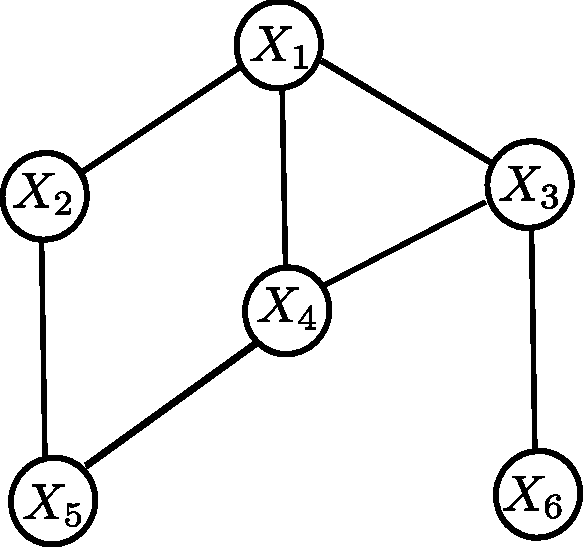
\includegraphics[width=4in]{figs/orig_graph}
          \end{column}

          \begin{column}{10in}
             Given: Graphical Model with known Parameters. \\
             \vspace{\itemlinespace}
             \textbf{Goal:} Estimate $\EE [h(X)]$ \\
             E.g.: $\mathbf{1}_A(x)$, $\sum_i X_i$ \\
             \vspace{\itemlinespace}
            Generate Samples: $\Xii{1}, \Xii{2}, \dots \Xii{N}$ \\
            \vspace{\itemlinespace}
            Empirical Estimator \\
              $\mu_0 = \frac{1}{N} \displaystyle\sum_{i=1}^N h(\Xii{i})$ \\
            \vspace{\itemlinespace}
            \textbf{Gibbs Sampling}--one way to generate samples.
          \end{column}

          \end{columns}
        
%         \insertparaspace
%           \semititle{Gibbs Sampling} \\ 
%           \insertlinespace
%           Current Sample: $\Xii{t}$\\
%           \vspace{\itemlinespace}
%           Sample: 
%           $\Xii{t+1}_1 \;|\; \Xii{t}_{2, 3, 4, 5, 6}$, \hspace{0.2in}
%           $\Xii{t+1}_2 \;|\; \Xii{t+1}_{1}, \Xii{t}_{3, 4, 5, 6}$,\hspace{0.2in}
%           $ \dots $ , \hspace{0.2in}
%           $\Xii{t+1}_6 \;|\; \Xii{t+1}_{1, 2, 3, 4, 5}$\\
%           \vspace{\itemlinespace}
%           Next Sample: $\Xii{t+1}$\\

        \insertparaspace
        \semititle{Blocked Gibbs Sampling} \\
        \vspace{\itemlinespace}
        \begin{columns}

        \begin{column}{5in}
          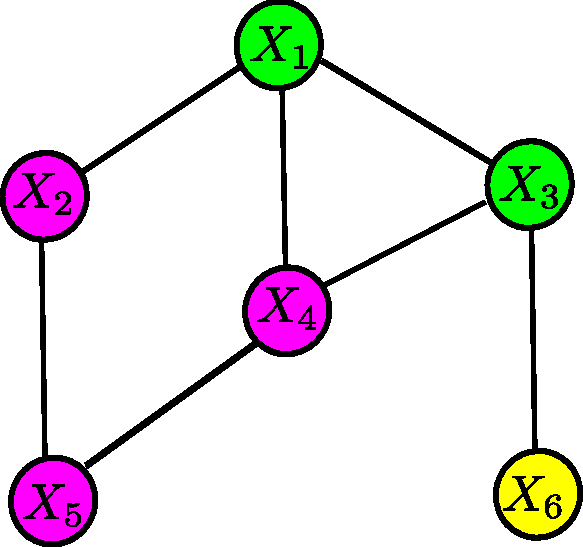
\includegraphics[width=4in]{figs/blocked_gibbs}
        \end{column}

        \begin{column}{5in}
            Current Sample: $\Xii{t}$\\
            \vspace{\itemlinespace}
            $\Xii{t+1}_{1,3} \;|\; \Xii{t}_{2, 4, 5, 6}$\\
            \vspace{\itemlinespace}
            $\Xii{t+1}_{2,4,5} \;|\; \Xii{t+1}_{1,3}, \Xii{t}_{6}$\\
            \vspace{\itemlinespace}
            $\Xii{t+1}_6 \;|\; \Xii{t+1}_{1, 2, 3, 4, 5}$\\
            \vspace{\itemlinespace}
            Next Sample: $\Xii{t+1}$\\
        \end{column}

        \begin{column}{5in}
            Why ?\\
            \vspace{\itemlinespace}
            Sampling is now more difficult. \\
            \vspace{\itemlinespace}
            BUT, Chain mixes faster $\implies$ better samples.
        \end{column}
        \end{columns}

        \insertparaspace
        \semititle{How to Block ?} \\
          \insertlinespace
          \newcommand{\localimgwidtha}{4in}
          \hspace{0.5in}
          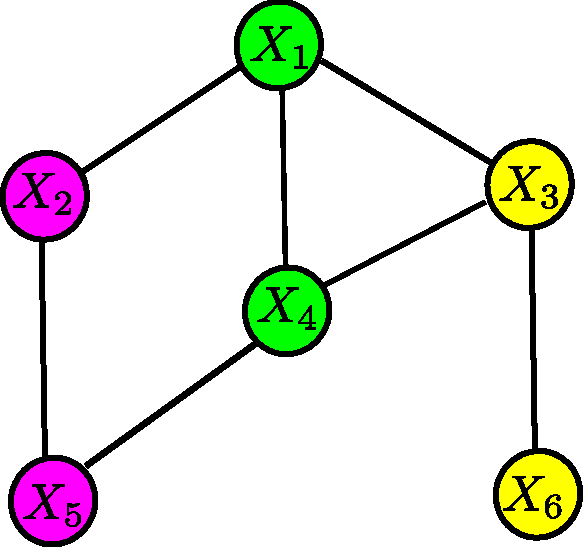
\includegraphics[width=\localimgwidtha]{figs/bg1} \hspace{0.5in}
          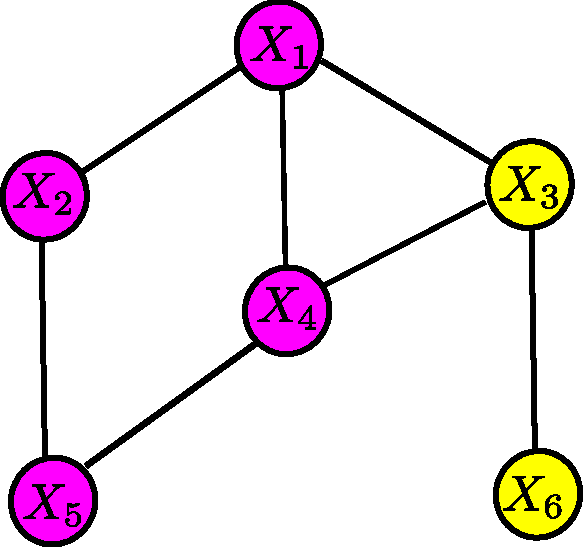
\includegraphics[width=\localimgwidtha]{figs/bg2} \hspace{0.5in} 
          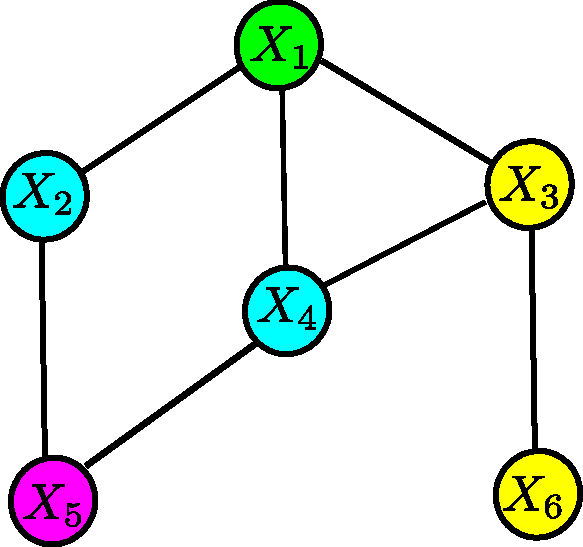
\includegraphics[width=\localimgwidtha]{figs/bg3} 
          \insertlinespace
        }
      \end{block}

      %-- Block 1-2
      \begin{block}{\Huge Strategy}
        { \huge
        \begin{itemize}
          \item We will focus only on \textbf{Tree Partitions}. \\
            \hspace{0.2in} - Otherwise Problem is too big. \\
            \hspace{0.2in} -  Inference on Trees is easy (Belief Propagation
                              converges in linear time).
          \item Will consider \textbf{correlations} between variables when
                developing tree blocks.
        \end{itemize}
        } 
      \end{block}

      %-- Block 1-3
      \begin{block}{\Huge Why Correlations ?}
      { \huge
%         \insertlinespace
% 
%         \semititle{MCMC Theory} \\
        \insertlinespace
        MC: $\Xii{1} \rightarrow \Xii{2} \rightarrow \dots \rightarrow \Xii{t}
          \rightarrow \Xii{t+1} \rightarrow \dots $, \hspace{0.2in}
        Eqlbm Distribtuion: $\pi$
        \insertlinespace

      $L_0(\pi) = \{ h:\Omega \rightarrow \RR :\; \EE_{\pi} h(X) = 0, \;
                        \VV_{\pi}h(X) < \infty \}$, \hspace{0.1in}
      $\langle h, g \rangle = \text{Covar}_\pi(h(X), g(X))$ \\
      $\big(L_0(\pi), \langle \cdot, \cdot \rangle \big)$ is a Hilbert Space.
      \insertlinespace

      Define $F:L_0(\pi) \rightarrow L_0(\pi)$,
        $ \,\; [Fh](z) = \EE[h(\Xii{1}) | \Xii{0} = z]$ \\
      \insertlinespace
 
      \textbf{Fact:}
%       Let $\Xii{0} \sim P^{(0)}$.
%       $P^{(n)}, \EE^{(n)} :$ n\textsuperscript{th} step evolution. \\
      % If $\|P^{(0)} - \pi\|_{\chi^2} < \infty $,
      $| \EE^{(n)} h(X) - \EE_\pi h(X) | \leq C \, \|F\|^n \, \|h\|$
      \insertlinespace

      $\|F\| = \sup_{f,g} \text{Corr}(f(\Xii{t+1}), g(\Xii{t}))$
      \insertlinespace

      Correlated Variables in different blocks $\implies$ successive
      samples correlated. \\
      \insertlinespace

        \textbf{So this is what we want:}  \\
        \insertlinespace
        \hspace{2in} 
        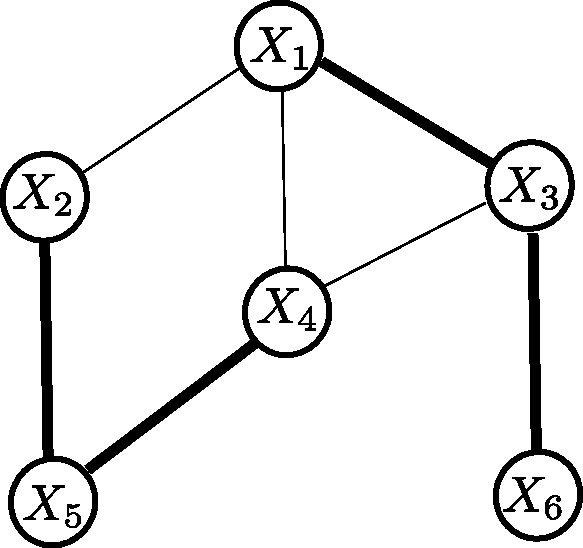
\includegraphics[width=4in]{figs/weighted} \hspace{0.4in}
        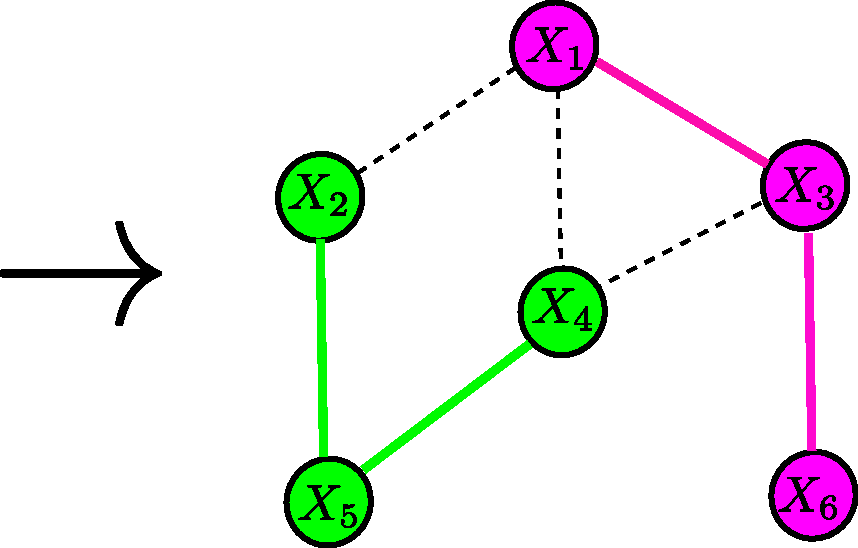
\includegraphics[width=6in]{figs/weighted_partition2}
      }
      \end{block}

    % End of Col 1 % -----------------------------------------------
    \end{column}%1

    %-- Column 2 ---------------------------------------------------
    %---------------------------------------------------------------
    \begin{column}{0.49\linewidth}
      %-- Block 2-?
      \begin{block}{Algorithms}
		For tree splitting, we consider algorithm from \cite{}. They
		greedily grows trees favoring vertices of low degree. We use
		its slightly simplified version as our baseline. We compared
		our algorithm, Greedy Edge Selection Algorithm, with the
		baseline under two different conditions.
		%\hsize .5\columnwidth
		\begin{columns}[t]
			%-- Column for algo
			\begin{column}{0.49\linewidth}

\begin{framed}
\noindent\textbf{Greedy Edge Selection Algorithm}
\begin{enumerate}
\item Construct an ordered list of edges, $E$, with $E[0]$ being the highest weight edge. Edges are vertex pairs $(i,j)$.
\item Initialize an all-zero $n$-dimensional integer list $V$ of vertex colors. \\
($V[i]$ is the color of vertex $i$, and $V[i]=0$ means that vertex $i$ has not yet been colored.)
\item Initialize $n$ empty vertex sets: $T_1,...,T_n$\\
(Logically, $T_i$ is the set of vertices labeled with color $i$.)
\item Initialize $unusedColor=1$.
\item For each edge $e=(i,j)$ in $E$,
\begin{itemize}
\item If $V[i]=V[j]=0$,
\begin{itemize}
\item Set $V[i]=V[j]=unusedColor$
\item Add $i,j$ to $T_{unusedColor}$
\item Increment $unusedColor$ by $1$
\end{itemize}
\item Else if $V[i]=0$ and $V[j]\notin getOtherNeighborColors(\{i\}, e)$,
\begin{itemize}
\item Set $V[i]=V[j]$
\item Add $i$ to $T_{V[j]}$
\end{itemize}
\item Else if $V[j]=0$ and $V[i]\notin getOtherNeighborColors(\{j\}, e)$,
\begin{itemize}
\item Set $V[j]=V[i]$
\item Add $j$ to $T_{V[i]}$
\end{itemize}
\item Else if  $V[i]\neq 0$ and $V[j]\neq 0$ and $V[i]\notin getOtherNeighborColors(T_j, e)$,
\begin{itemize}
\item For each $k\in T_j$, set $V[k]=V[i]$
\item Set $T_i=T_i\cup T_j$
\item Set $T_j=\emptyset$
\end{itemize}
\item Otherwise do nothing
\end{itemize}
\item For each vertex $i$, if $V[i]=0$, set $V[i]=unusedColor$, $unusedColor++$
\item Output $\{T_j:T_j\neq\emptyset\}$
\end{enumerate}
\end{framed}

\begin{framed}
\noindent\textbf{Greedy Tree Growing Algorithm} % \cite{rivasseau2005jungle}}
\begin{enumerate}
\item Initialize $i=0$ and $V$ to the vertex set.
\item While $V\neq\emptyset$
\begin{itemize}
\item Select $v\in V$
\item Start a new tree $T_i$ and a priority queue $Q_i$. Add $v$ to $Q_i$
\item While $Q_i\neq\emptyset$
\begin{itemize}
\item Pop $u$ from $Q_i$.
\item Initialize $neighborsInT=0$.
\item For all $v\in T_i$, if $u\in N(v)$, increment $neighborsInT$
\item If $neighborsInT\le1$,
\begin{itemize}
\item Add $u$ to $T_i$ and remove $v$ from $V$
\item Add $N(u)$ to $Q_i$.
\end{itemize}
\end{itemize}
\end{itemize}
\item Return $\{T_i\}$
\end{enumerate}
\end{framed}

			\end{column}
			%-- Column for algo
			\begin{column}{0.49\linewidth}

\begin{figure}
	\centering
	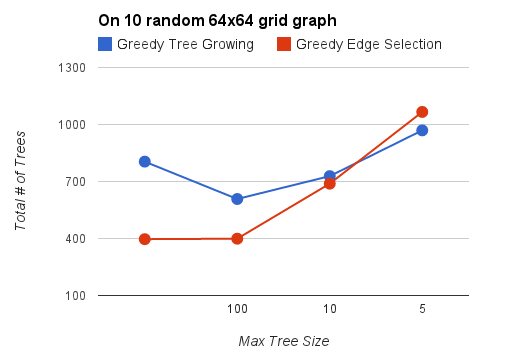
\includegraphics[width=\columnwidth]{TotalTrees-Vs-MaxTreeSize.png}
\end{figure}
\vspace{-0.4in}
\begin{figure}
	\centering
	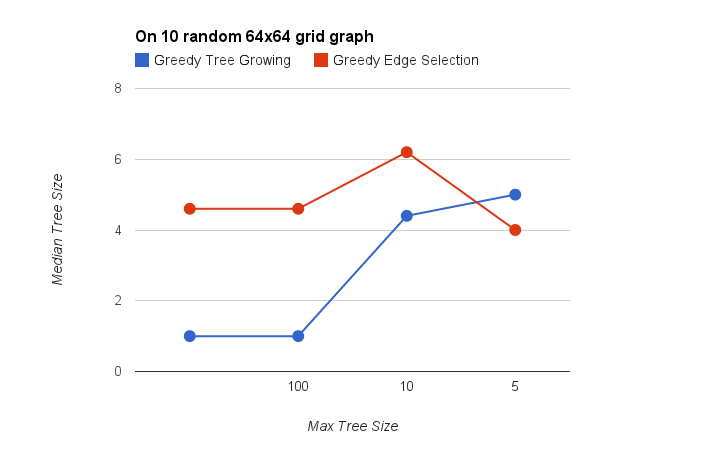
\includegraphics[width=\columnwidth]{MedianTreeSize-Vs-MaxTreeSize.png}
\end{figure}
\vspace{-0.4in}

%			We consider a tree-splitting algorithm to be good if it
%			can give us a small number of total trees and if the
%			median size of the trees are relatively small. 
			
			With no limit on the max tree size (the leftmost dots),
			Greedy Edge Selection Algorithm performs much better than
			Greedy Tree Growing Algorithm. 

			But when as the limit of max tree size goes down, Greedy
			Tree Growing Algorithm caught up with Greedy Edge
			Selection Algorithm.
			\end{column}
		\end{columns}

      \end{block}

      %-- Block 2-1
      \begin{block}{Lists}
        \begin{itemize}
          \item You can make
          \item lists, that
          \item allow people to see quickly
        \end{itemize}
      \end{block}

      %-- Block 2-2
      \begin{block}{Math}
        Include math within the text is as simple as $1+1=2$.  You can also
        highlight more important equations like this:
        \begin{equation*}
          \int_0^1\sin(x)+\cos^2(x)+\alpha x~d\!x
        \end{equation*}
      \end{block}


      %-- Block 2-3
      \begin{block}{Pictures}
        \begin{figure}[htb]
          \centering
%           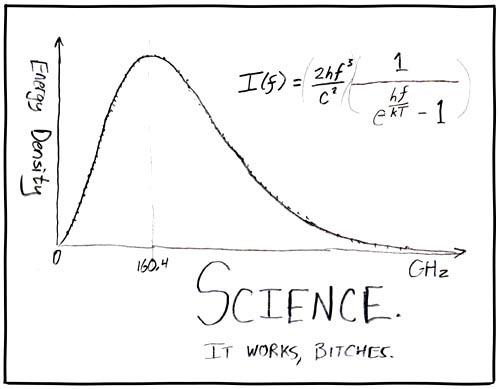
\includegraphics[width=.6\columnwidth]{science}
        \end{figure}
      \end{block}

      %-- Block 3-1
      \begin{block}{Experiments}
        Remember to put lots of figures on your poster... Nobody reads anymore!
      \end{block}

      %-- Block 3-2
      \begin{block}{Conclusion}
        Much less annoying than PowerPoint.  Copy and Paste from your
        document. Overall, a great idea!
      \end{block}

    \end{column}%2

% I think we should do just 2 columns
%     %-- Column 3 ---------------------------------------------------
%     \begin{column}{0.32\linewidth}
% 
%     \end{column}%3

  \end{columns}
\end{frame}
\end{document}
